%%%%%%%%%%%%%%%%%%%%%%%%%%%%%%%%%%%%%%%%%%%%%%%%%%
%% Layer Overview
%%%%%%%%%%%%%%%%%%%%%%%%%%%%%%%%%%%%%%%%%%%%%%%%%%


%%%%%%%%%%%%%%%%%%%%%%%%%%%%%%%%%%%%%%%%%%%%%%%%%%
%% Subsystem X - Template
%%%%%%%%%%%%%%%%%%%%%%%%%%%%%%%%%%%%%%%%%%%%%%%%%%

% \subsection{Subsystem X}
% Descibe at a high level the purpose and basic design of this subsystem. Is it a piece of hardware, a class, a web service, or something else? Note that each of the subsystem items below are meant to be specific to that subystem and not a repeat of anything discussed above for the overall layer.

% \begin{figure}[h!]
% 	\centering
%  	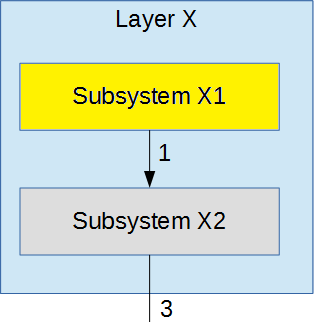
\includegraphics[width=0.60\textwidth]{images/subsystem}
%  \caption{Example subsystem description diagram}
% \end{figure}

% \subsubsection{Subsystem Hardware}
% A description of any involved hardware components for the subsystem.

% \subsubsection{Subsystem Operating System}
% A description of any operating systems required by the subsystem.

% \subsubsection{Subsystem Software Dependencies}
% A description of any software dependencies (libraries, frameworks, design software for mechanical parts or circuits, etc) required by the subsystem.

% \subsubsection{Subsystem Programming Languages}
% A description of any programming languages used by the subsystem.

% \subsubsection{Subsystem Data Structures}
% A description of any classes or other data structures that are worth discussing for the subsystem. For example, data being transmitted from a microcontroller to a PC via USB should be first be assembled into packets. What is the structure of the packets?

% \subsubsection{Subsystem Data Processing}
% A description of any algorithms or processing strategies that are worth discussing for the subsystem. If you are implementing a well-known algorithm, list it. If it is something unique to this project, discuss it in greater detail.



The Pathfinding Subsystem controls the rover's movement, by utilizing the rover's LIDAR to create a map of the terrain. The subsystem will than create a costmap grid, and than applying an A* pathfinding algorithm to find the most efficient and safest path.

\subsection{LIDAR}
The LIDAR subsystem is a hardware component responsible for environmental perception and obstacle detection. It operates by emitting laser pulses and measuring the time it takes for them to reflect off surrounding objects, generating a point cloud representation of the environment. This data enables the differential mobile robot to construct a real-time map, detect obstacles, and facilitate autonomous navigation. The LIDAR subsystem integrates with the robot's path planning and localization systems, providing critical spatial awareness for efficient and collision-free movement.

\begin{figure}[h!]
	\centering
 	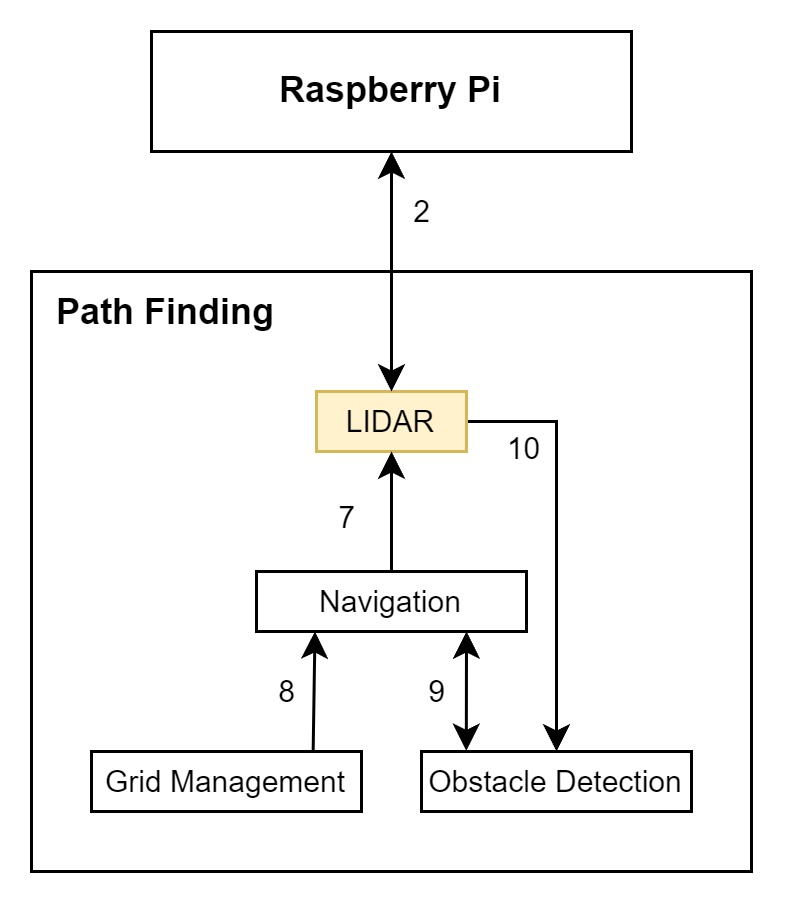
\includegraphics[width=0.60\textwidth]{images/pathfinding/1_lidar.jpg}
 \caption{Pathfinding Layer - LIDAR Subsystem}
\end{figure}


\subsubsection{Subsystem Hardware}
Slamtec RPLIDAR A1 - 360-degree laser range scanner. With a maximum range of 100 meters and a sampling frequency of a little over 2500 samples a second, measures distances and angles to create a 2D cloud point representation of the surroundings.

\subsubsection{Subsystem Operating System}
The LIDAR is compatible with both Windows and Linux.

\subsubsection{Subsystem Dependencies}
The LIDAR system utilizes the RPLIDAR SDK developed by Slamtec to facilitate its operation and data processing.

\subsubsection{Subsystem Programming Languages}
The RPLIDAR SDK developed by Slamtec is primarly written in C++.

\subsubsection{Subsystem Data Structures}
The RPLIDAR will be used to make a linked list of all data points so that it can be transferred to the navigation system and let it know where any obstacles are.

\subsubsection{Subsystem Data Processing}
The LIDAR system acquires raw data points in the form of a point cloud by measuring the distances between emitted laser pulses.

\newpage

\subsection{Navigation}
The Navigation subsystem software integration that allows a Raspberry Pi 5 to compute and execute navigation commands for a robot. It enables autonomous movement by processing sensor data, calculating an optimal path, and sending motor control signals to drive the robot accordingly.

\begin{figure}[h!]
	\centering
 	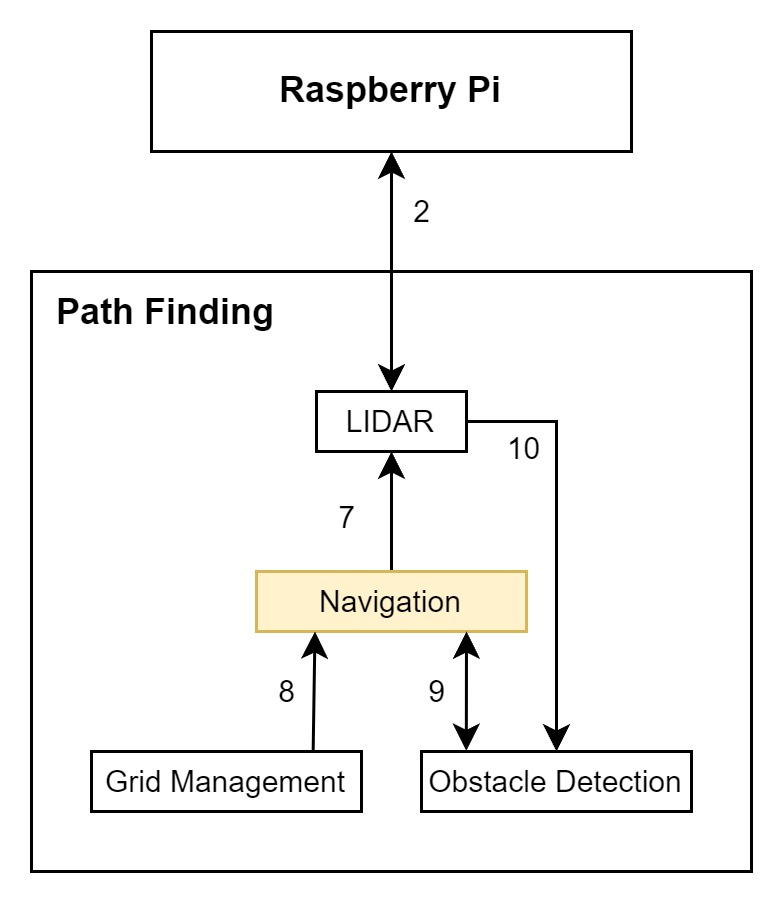
\includegraphics[width=0.60\textwidth]{images/pathfinding/2_navigation.jpg}
 \caption{Pathfinding Layer - Navigation Subsystem}
\end{figure}

%\subsubsection{Subsystem Hardware}
%The navigation software will be housed on the Raspberry Pi 5.
\subsubsection{Subsystem Operating System}
The navigation subsystem will be run on ROS2 Jazzy which requires Ubuntu 24.04 (Noble Numbat) or higher for compatibility. 
\subsubsection{Subsystem Software Dependencies}
The Navigation Subsystem uses Nav2 and ROS2 to develop the pathfinding algorithm and design the path for the rover to follow, and ROS2 to manage the robot's movements.

\subsubsection{Subsystem Programming Languages}
Nav2 is primarily implemented in C++ to ensure optimal compatibility with ROS2, which is also C++-based. However, it also provides a Python API for additional flexibility.
%\subsubsection{Subsystem Data Structures}
\subsubsection{Subsystem Data Processing}
The pathfinding subsystem employs the A* algorithm due to its ability to determine the most optimal path while maintaining lower computational overhead compared to alternative pathfinding methods.

\newpage

\subsection{Grid Management}
The Grid Management subsystem operates on ROS2 Jazzy, which will be hosted on the Raspberry Pi 5.

\begin{figure}[h!]
	\centering
 	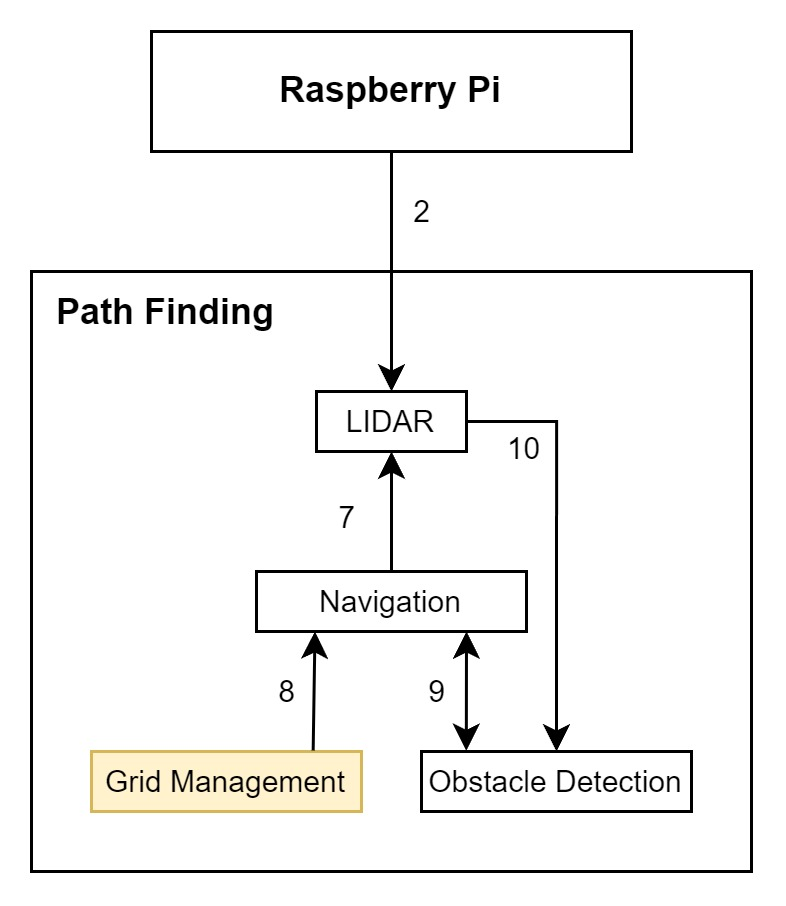
\includegraphics[width=0.60\textwidth]{images/pathfinding/3_grid.jpg}
 \caption{Pathfinding Layer - Grid Management Subsystem}
\end{figure}


%\subsubsection{Subsystem Hardware}
%The Grid Management runs on Ros2 Jazzy which will be stored on the Raspberry Pi 5.
%\subsubsection{Subsystem Operating System}
%The Grid Management Subsystem will operate on ROS2 Jazzy, which requires Ubuntu 24.04 or later
\subsubsection{Subsystem Programming Languages}
The Grid Management Subsystem creates a costmap using C++.
% \subsubsection{Subsystem Data Structures}

\newpage

\subsection{Obstacle Detection}

The Obstacle Detection subsystem leverages the costmap generated by the Grid Management Subsystem to assess the robot's environment. It assigns a numerical value to each grid cell based on the proximity of surrounding objects, with higher values indicating closer objects and lower values representing areas free from obstacles.


\begin{figure}[h!]
	\centering
 	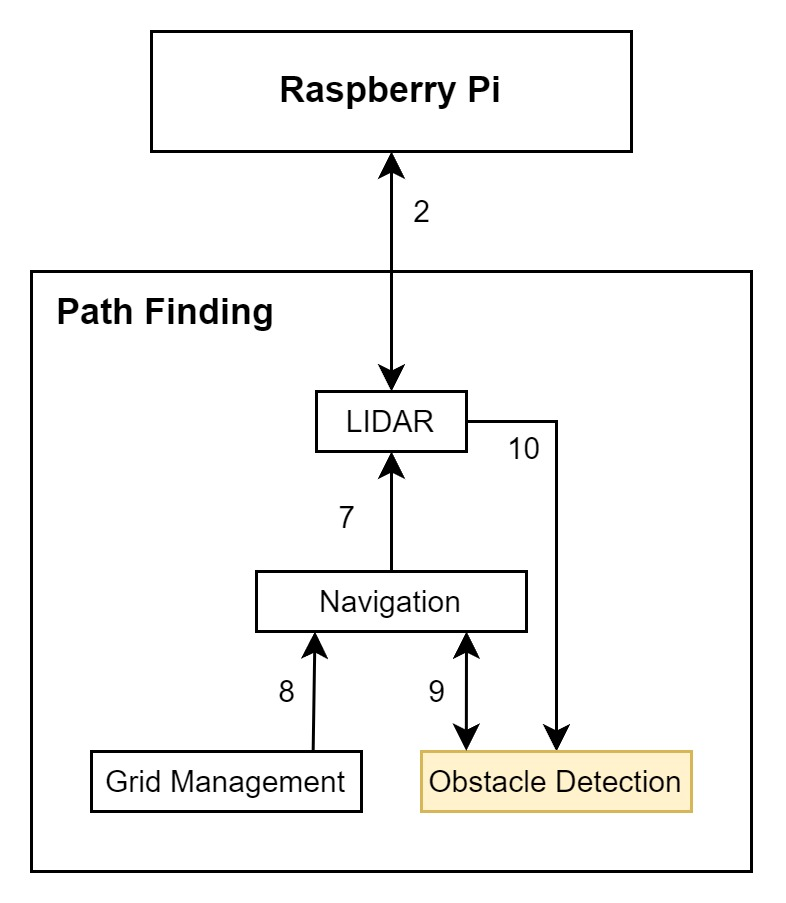
\includegraphics[width=0.60\textwidth]{images/pathfinding/4_obstacle.jpg}
 \caption{Pathfinding Layer - Obstacle Detection Subsystem}
\end{figure}

%\subsubsection{Subsystem Hardware}


\subsubsection{Subsystem Operating System}
%A description of any operating systems required by the subsystem.
ROS2 Jazzy requires Ubuntu 24.04 (Noble Numbat) or higher for compatibility.
\subsubsection{Subsystem Software Dependencies}
%A description of any software dependencies (libraries, frameworks, design software for mechanical parts or circuits, etc) required by the subsystem.
The Grid Management Subsystem uses Nav2 to develop the pathfinding algorithm and design the path for the rover to follow, and ROS2 to manage the robot's movements.

\subsubsection{Subsystem Programming Languages}
%A description of any programming languages used by %the subsystem.
Nav2 is primarily in C++, so it can better configure with ROS2 which is also in C++, but Nav2 does allow for a Python API.

%\subsubsection{Subsystem Data Structures}
%A description of any classes or other data structures that are worth discussing for the subsystem. For example, data being transmitted from a microcontroller to a PC via USB should be first be assembled into packets. What is the structure of the packets?

\subsubsection{Subsystem Data Processing}
%A description of any algorithms or processing %strategies that are worth discussing for the %subsystem. If you are implementing a well-known %algorithm, list it. If it is something unique to this %project, discuss it in greater detail.
The pathfinding subsystem utilizes the A* pathfinding for its ability to find the most optimal path while being less computationally inexpensive than the other pathfinding subsystems. 

